\chapter{Goals}

\section{Introduction}
Modern machine learning models based on deep neural networks are achieving remarkable performance on many fields, including medical image analysis. In comparison
with classic machine learning technologies like decision trees, it is much harder to explain how these neural network came to its conclusion, because it uses thousands to millions of training parameters.

In recent years, many methods for the interpretability of deep (convolutional) neural networks have been proposed, e.g. LIME\cite{ribeiro2016should}, RISE\cite{Petsiuk2018rise}, Grad-CAM\cite{selvaraju2017grad} or DeepLIFT \cite{shrikumar2017learning}.

\begin{figure}[h]
\centering
\caption{Examples of some interpreatbility methods for image classification \cite{visualattribution}}
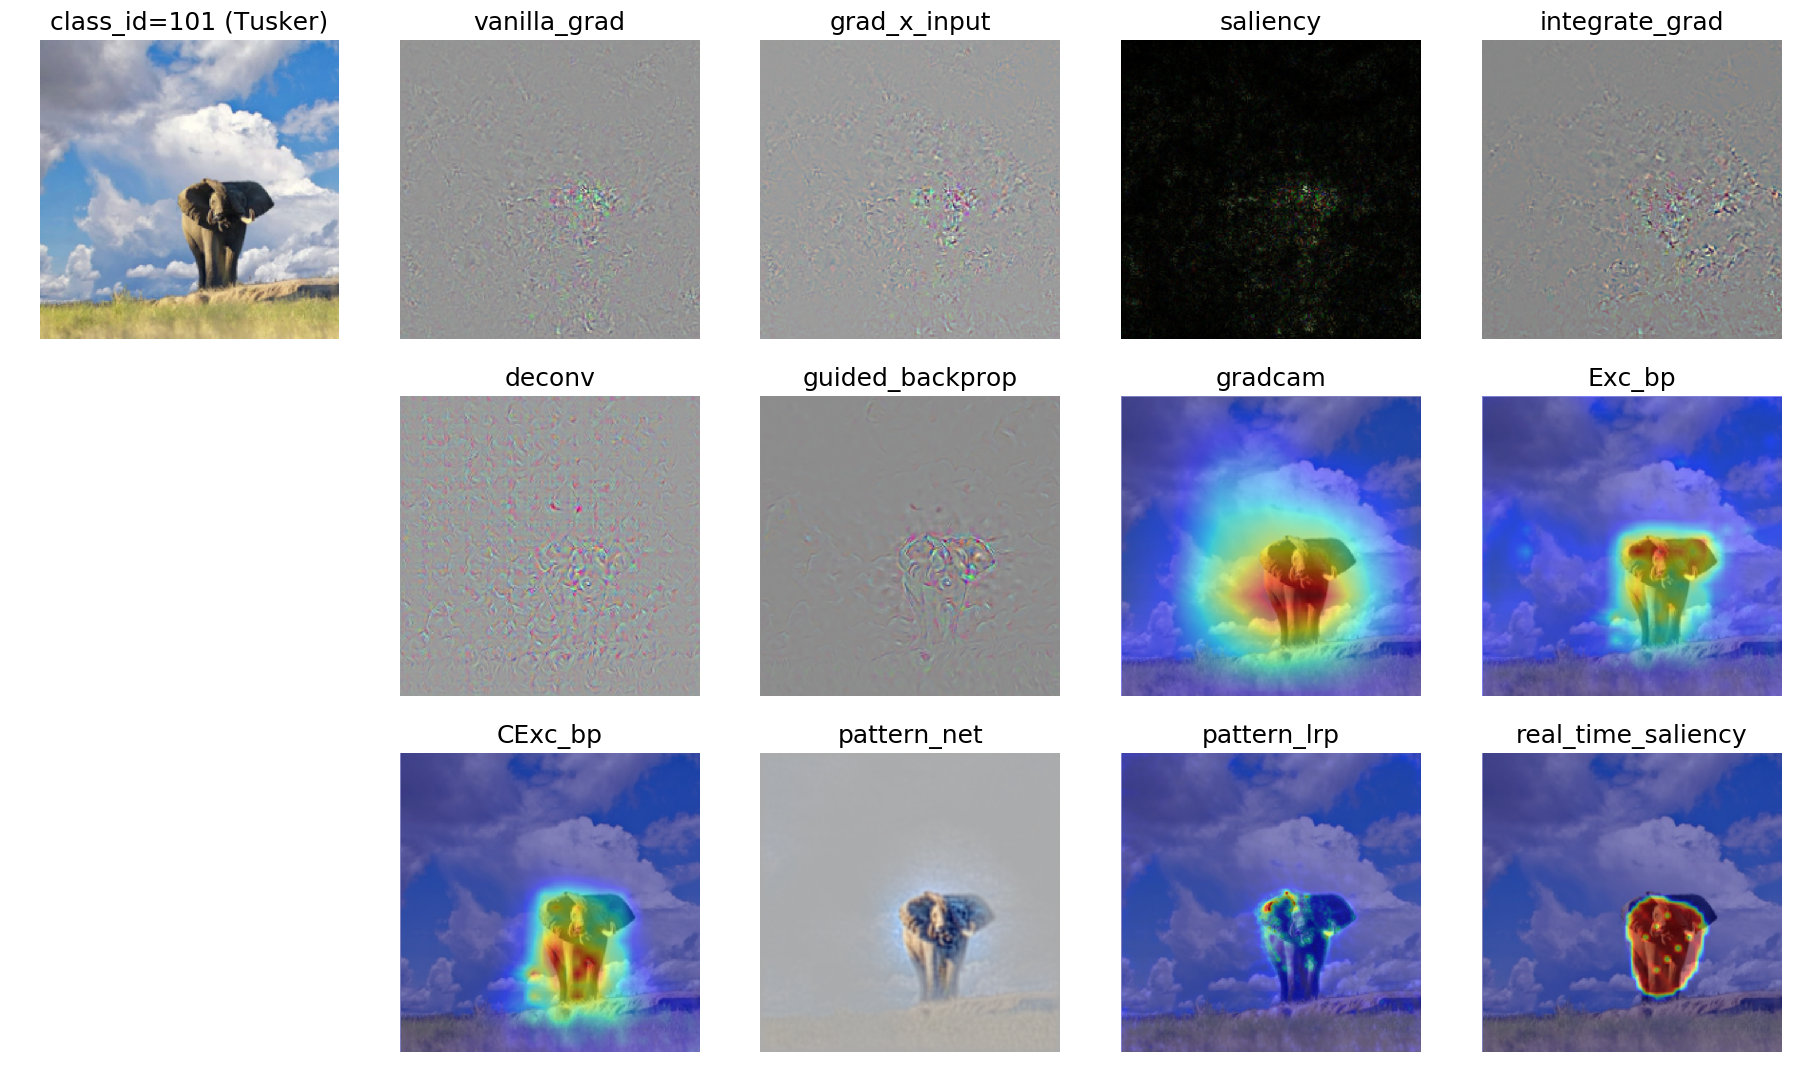
\includegraphics[width=14cm]{images/tusker_saliency.png}
\end{figure}

These methods focus on providing explanations and interpretability of classification problems for datasets like ImageNet or MNIST. What has not yet been researched much is the interpretability of image segmentation tasks. On many image segmentation tasks, interpretability based image regions like Grad-CAM (see image above) does not make that much sense, because the segmentation already returns a region of an image.

\begin{figure}[H]
\centering
\caption{Image segmentation on MRI scans of the brain\cite{soltaninejad2017automated}}
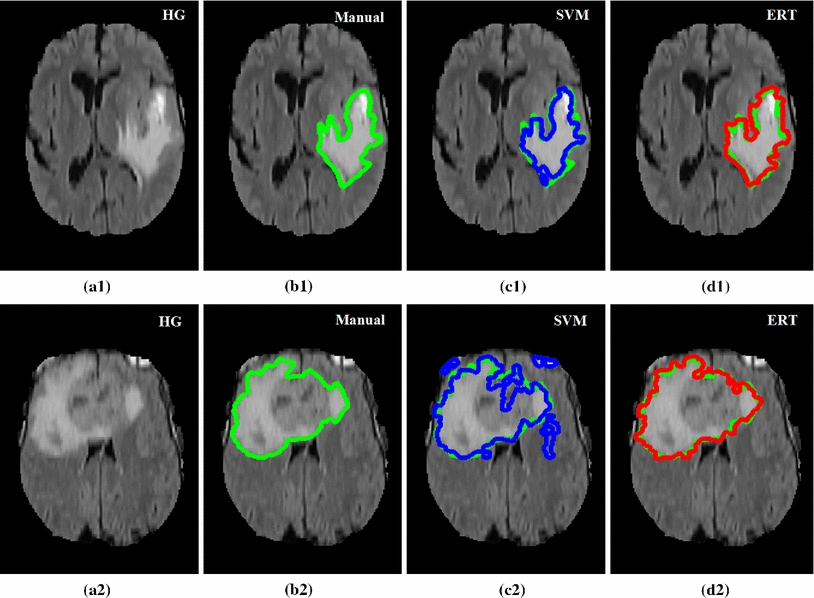
\includegraphics[width=10cm]{images/brain_segmentation.jpg}
\end{figure}

On other problems like finding and segmenting brain tumors on MRI images, medical professionals do not only look at the exact region where a tumor resides, but also at other regions of the brain. On the upper row of the scan above it is cleary visible that the tumor on the right side is extending the space used for the right half of the brain, and therefore many brain features are not symmetrical any longer. A neural network trained on this task should also use these cues to correctly segment the tumors. 

The main goal of this thesis is to provide such a tool by modifying existing interpretability methods to work on image segmentation.

\section{Planning}
All steps described here are prerequisites for the next step if not noted otherwise.

\subsection{NIH Chest X-ray}
To get a general overview how the different interpretability methods work, we plan to build a model for a medical imaging task and apply some of the more commonly used methods on it. We will also search for existing pretrained models to complete this work faster and/or to have a more accurate model. The model will reuse an existing convolutional neural network architecture, e.g. ResNet or Inception.

The dataset selected for this task is the NIH Chest X-ray dataset \cite{wang2017chestx}. It contains 120.000 grayscale x-ray scans of chests and labels ranging from no findings to one or more diagnoses.

After building the model, we evaluate some of the common methods on the trained models. We want to determine which methods are independent of the used network architecture (methods that view the model as a black box). We also want to find implementations of the methods written for PyTorch or alternatively estimate how easy the methods could be ported to PyTorch. The last step is to show how the output of the method looks like and (optionally) check with a medical professional which output they think would be most helpful for the interpretability of a method.

\subsection{Brain tumors}
To build the methods to interpret image segmentation tasks, we need a real world task. Brain tumor segmentation is an interesting problem in the medical image field. Segmenting brain tumors manually is a tedious process, because MRI machines generate many slices of the brain which then have to be looked at one by one. Automating the process with machine learning will give medical professionals more time to do other tasks and also gives them more confidence in their manual work when supported by an automated model.

To build a working machine learning model, some medical background is required. We will investigate what types of brain tumors exits, how do they look like on a scan and what scanner types exists (MRI/PET/CT). We also investigate how a tumor looks like on a specific scanner type.

\subsection{The BraTS 2018 dataset}
The BraTS\cite{menze2015multimodal} dataset contains MRI scans of the human brain and segmentation labels for found tumors in the scans.
The scan is 3D, saved as horizontal 2D slices. Every slice has four different black/white channels, each with a different setting of the MRI scanner.
There are four different labels for every slice, representing 4 different sizes of a tumor.

The tasks for this step is to figure out the data format of the dataset and then load the dataset into memory. Displaying some slices will show if the data was loaded correctly. Next, we extract multiple slices per scanned brain. We only use slices which contain visible tumors. This way we have 2D images we can feed into the encoder convolutional neural network of the U-net.

The next step is loading the labels of the data. As recommended by Alain Jungo of the Universität Bern, we will merge the two innermost region labels into one label and discard the other two labels.

\subsection{Model for the BraTS dataset}
A widely used architecture for segmentation (especially in the medical imaging field) is the U-Net\cite{ronneberger2015u} architecture.

\begin{figure}[H]
\centering
\caption{The U-Net architecture}
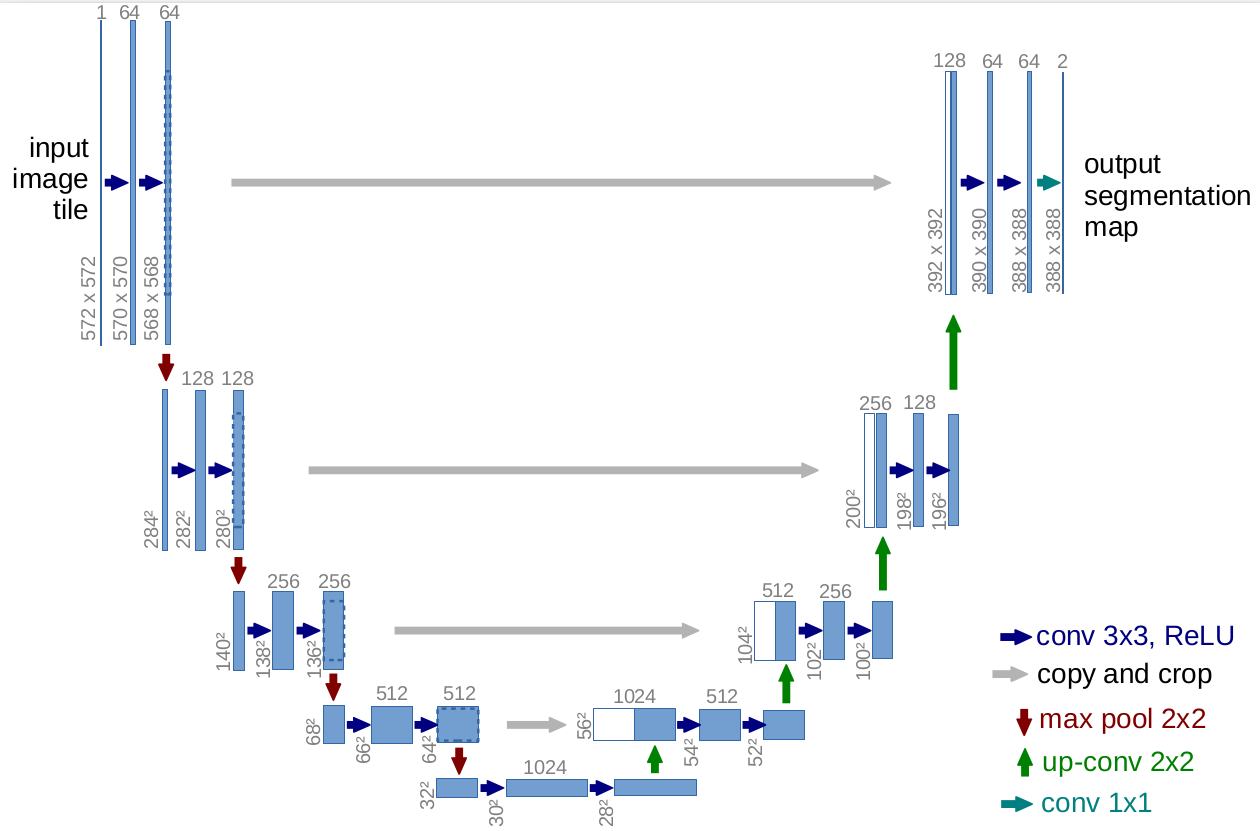
\includegraphics[width=10cm]{images/unet.png}
\end{figure}

The architecture uses an "encoder" network on the left side which generates features. A standard convolutional neural network can be used as an encoder. On the right side, instead of a linear layer mapping features generated from the convolutions to classes, a "decoder" network is used. The decoder network generates the output segmentation pixels based on the features extracted by the encoder.

We will build a U-Net using a standard convolutional neural network architecture. The fast.ai library contains a dynamic U-Net Python class which can automatically generate a the decoder part of a U-Net by analyzing the CNN. We will evaluate if this works good enough or if a custom architecture is required.

\subsection{RISE}
Randomized Input Sampling for Explanations (RISE) is a interpretability method that uses the model as a blackbox. It does not need to know anything about the underlying machine learning model, it only needs access to the input image and the probabilities of the output classes.

RISE generates a series of masks which get applied to the input image. The modified image is then run through the model and the changed probabilities of the output classes are recorded. From the probabilities of the different masks, a heatmap is generated which shows which parts of the image influence the correct classification of the image the most.

To use RISE for image segmentation, we have to find a way to replace the class probabilities with the segmentation pixels. This is the main research work for this thesis.

\subsection{Other blackbox model methods (Optional}
There are other blackbox methods (e.g. LIME\cite{ribeiro2016should}) which work similar to RISE. If a successful method is found to apply RISE to image segmentation tasks, modifying these other methods to also work for segmentation should not be a major problem.

Building a high quality solution with RISE has a higher priority than adding additional methods.

\subsection{Grad-CAM Method}
The Grad-CAM\cite{selvaraju2017grad} (Gradient-weighted Class Activation Mapping) is a whitebox method which uses the parameters of a learned model to output a heatmap for a specific image classified by the network.

Grad-CAM is a widely used method with many high quality implementations which also generated a easy to understand output which can be used by medical professionals.

As with RISE, Grad-CAM is built for image classification tasks. Because the encoder part of a U-Net is a standard convolutional neural network, it should be possible to apply Grad-CAM on this part of the U-Net. If and how this is possible is is the main research topic for this thesis.

\subsection{Other whitebox model methods (Optional}
As described above, there are many whitebox model methods which can be applied to this problem. If we can find a solution how to apply Grad-CAM, using other methods like PatternNet or 

\subsection{Library}
If we succeed with modifying the methods to work with image segmentation tasks, we plan to build a Python library which allows to easily apply the methods to other datasets by its users. The library should be usable with PyTorch models. Documenting the library (e.g. on readthedocs.io) is essential for potential users, as are examples how to use the library which can be extracted from the thesis source code.

Also planned is to publish the library on PyPI and conda-forge, so researchers can install the library in their environments.

\section{Infrastructure and technology}
This work will use the PyTorch\cite{paszke2017automatic} deep learning library. Most newer machine learning papers are written with PyTorch, because it is considered easier to learn and more powerful than Keras and PyTorch\cite{pytorchvstensorflow}.

Other machine learning libraries will be used on demand, for example:

\begin{tabular}{|p{3cm}|p{12.5cm}|}
    \hline
    \textbf{Library} & \textbf{Description} \\ \hline
    Scikit & Diverse kit of machine learning libraries \\ \hline
    Matplotlib & Library to generate graphs \\ \hline
    PIL/Pillow & Image manipulation library \\ \hline
    NumPy & Matrix manipulation library \\ \hline
    pandas & Dataframe library \\ \hline
    torchvision & PyTorch extension for computer vision problems. Contains models for common architectures and pretrained parameters for these networks. Also contains tools for data augmentation. \\ \hline
\end{tabular}

The development of the system will take place inside Jupyter notebooks. Jupyter notebooks allow a very fast test and development cycle. The notebook server will be running on a powerful desktop computer of the author which is exposed to the internet, so the computational power is always available independent of the work location.

In addition, the GPU servers from the Berner Fachhochschule (NVIDIA DGX-1, 4x Tesla V100) and from the Institute for Surgical Technology and Biomechanics of the Universität Bern (Unknown number and type of GPUs) are available. Because the setup cost to use these servers is quite high, the usage of these systems is optional and time will only be invested if the learning speedup is worth the additional setup time.

\pagebreak
\section{Gantt chart}

The following Gantt chart shows the time planning for the thesis. The light blue charts represent optional goals, which also function as reserve time if another goal needs more time than anticipated.

\begin{ganttchart}[
bar/.style={fill=bar},
vgrid,
hgrid,
milestone/.append style={anchor=east,xshift=-1pt,fill=milestone,shape=circle,draw=milestone,},
title height=1.0,
x unit=7mm,
y unit title=8mm,
y unit chart=8mm,
]{10}{25}
    \gantttitle{Calendar weeks 2019}{16} \\
    \gantttitlelist{10,...,25}{1} \\
    \ganttbar[bar/.append style={fill=fulltimebar}]{Full-time work on thesis}{10}{15} \ganttnewline

    \ganttbar{Chest X-Ray}{10}{11} \ganttnewline
    \ganttbar{Investigate interpretability methods}{11}{11} \ganttnewline
    \ganttmilestone{Goals definied}{11} \ganttnewline
    \ganttbar{U-Net model for BraTS}{12}{12} \ganttnewline
    
    \ganttbar{RISE}{13}{14} \ganttnewline
    \ganttbar{Grad-CAM}{14}{15} \ganttnewline
    
    \ganttbar[bar/.append style={fill=optionalbar}]{Additional blackbox methods}{16}{18} \ganttnewline
    \ganttbar[bar/.append style={fill=optionalbar}]{Additional whitebox methods}{16}{18} \ganttnewline
    \ganttbar{Python library}{19}{19} \ganttnewline
    
    \ganttbar{Finish text}{20}{22} \ganttnewline

    \ganttmilestone{Draft paper done}{22} \ganttnewline
    \ganttbar{Presentation preparation}{23}{24} \ganttnewline
    \ganttmilestone{Deadline paper \& Presentation}{24} \ganttnewline
    \ganttmilestone{Defense}{25}
\end{ganttchart}